\documentclass[ngerman]{article}
\usepackage[utf8]{inputenc}
%\usepackage[T1]{fontenc}
\usepackage{lmodern}
\usepackage{amssymb,amsmath}
\usepackage{ifxetex,ifluatex}

\usepackage[german]{todonotes}
\usepackage[hidelinks]{hyperref}

\usepackage{algorithm}
\usepackage{algorithmic}

% Folgende Zeilen waren im orignalen Markdown Export, ich hab sie erstmal auskommentiert.
%\setlength{\parindent}{0pt}
%\setlength{\parskip}{6pt plus 2pt minus 1pt}
%\setlength{\emergencystretch}{3em}  % prevent overfull lines
%\setcounter{secnumdepth}{0}

\title{180: Testen, Verifizieren, Analysieren}
\author{Ricarda Schüler und Stefan Bunk}
\date{24.01.2016}

\begin{document}

\listoftodos
\tableofcontents

\section{Überblick über die Anwendung}
\label{sec:ueberblick}

\subsection{Sinn und Zweck}

180 ist eine Web-Anwendung, die Bachelor-Studenten des Hasso-Plattner-Instituts dabei unterstützt, eine korrekte Belegung zu finden, und somit ihr Bachelorstudium erfolgreich zu beenden.
Durch die Wahl von unterschiedlichen Vertiefungsgebieten sowie die Tatsache, dass viele Veranstaltungen mehreren Vertiefungsgebieten zuordenbar sind, kann es schwierig werden, eine korrekte Belegung zu finden.

Der Name 180 stammt von den 180 Leistungspunkten, die erforderlich sind, um das Bachelorstudium erfolgreich abzuschließen.
Es existiert desweiteren ein Schwesterprojekt namens 120, das von Masterstudenten des HPIs genutzt werden kann, und das den gleichen Zweck verfolgt.
Dieses Dokument befasst sich allerdings nur mit 180.

\subsection{Entwicklungsparadigma und Programmiersprache}

\begin{itemize}
    \item Javascript
    \item no TDD
\end{itemize}

\subsection{Anforderungen, Spezifikation und Dokumentation?}

Die Anwendungen wurde aus dem persönlichen Bedarf heraus entwickelt, und es gab keinen externen Auftraggeber.
Der Entwickler war Stefan Bunk.

Obwohl es damit keine Spezifikation im klassischen Sinne gibt, sind dennoch die zu implementierenden Regeln genau festgelegt:
In der \todo{TODO: Titel Studienordnung}, der Studienordnung für den Bachelor- und Masterstudiengang am HPI.

\begin{itemize}
    \item
        Spezification: Studienordnung des HPI -- \todo{Vorstellung Regeln, Vertiefungsgebiete}
    \item
        Vertrauliche Daten: kein Sharen über das Internet
    \item
        Waterfall
\end{itemize}

\subsection{Aktueller Teststatus, Ziele der Tests? Bug Repositories?}

\begin{itemize}
    \item
        keine automatisiertes Tests
    \item
        manuelle Tests
    \item
        \url{https://github.com/knub/onehundredandeighty/issues?q=is:issue}
\end{itemize}

Analyse der bisherigen Issues:

\begin{itemize}
    \item
        2 * Feature-Requests nach Berechnung der Gesamtnote -- abgelehnt
    \item
        1 * Syntaxfehler, der die Ausführung des Programmes unmöglich machte
    \item
        1 * Feature-Request nach variabler Anzahl der Semester, der teilweise umgesetzt wurde.
    \item
        1 * \href{https://github.com/knub/onehundredandeighty/pull/5}{\underline{Issue}} aufgrund einer Änderung
        der Wirtschaftsvorlesung, die statt zwei 3-LP-Veranstaltungen ab dem WS11/12 als eine
        6-LP-Veranstaltung angeboten wurden.
\end{itemize}

\subsection{Rollenverteilung der Tester}

\begin{itemize}
    \item 1 Developer and User
    \item 2 User
\end{itemize}

\subsection{Stakeholders}

\begin{itemize}
    \item Students
    \item HPI Studienverwaltung
\end{itemize}

\section{Initialer Test Plan}

\subsection{Wann beginnen Verifikation und Validation? Wann sind sie beendet?}

\subsubsection{Validation: Die richtige Anwendung bauen!}

180 wurde entwickelt unter der Annahme, dass es für jeden Studenten kompliziert ist, sein Studium entsprechend der Studienordnung zu planen.
Insbesondere die Beachtung aller Regeln der Vertiefungsgebiete ist kompliziert und erfordert mehrfaches Überprüfen aller Bedingungen.
\todo{Beispiel hinzufuegen}

In diesem Bereich lässt die Studienordnung einen großen Spielraum zu, der entsprechend der eigenen Interesseren ausgefüllt werden kann aber auch muss.
Die Menge aller gültigen Belegungen ist damit sehr groß, übersieht man allerdings eine einzige Bedingung führt dies zu einem ungültigen Belegungsplan.
Merkt man dies nicht rechtzeitig, muss im schlimmsten Fall ein weiteres Semester im Bachelorstudium eingeplant werden.

Daher ist die Idee von 180 diese manuelle und fehleranfällige Prüfung zu automatisieren.
Da die Regeln der Studienordnung sich nicht schnell ändern (mehr zu möglichen Änderungen der Studienordnung weiter unten \todo{vielleicht als Footnote}), genügt es, die Regeln einmal korrekt zu implementieren.
Daher ist dies auch der zentrale Punkt der Validierung:
Die Anwendung muss genau dann ausgeben, dass ein Belegungsplan valide ist, wenn er nach den Paragraphen der Studienordnung korrekt ist.
Kann die Anwendung dies nicht garantieren, ist sie nahezu nutzlos.
Wird der Anwendung nicht vertraut, wird sie niemand nutzen, da sowieso eine manuelle Prüfung notwendig wird.

\begin{itemize}
    \item nur Wünsche von Studenten erfüllt, wenn komplette Studienordnung richtig abgedeckt ist
    \item Start: PEM, End:
\end{itemize}

\subsubsection{Verifikation: Die Anwendung richtig bauen!}

Um die Anwendung richtig zu bauen, folgt man der Spezifikation.
In diesem Fall gibt es keine interne, von den Entwicklern gemeinsam mit den Anwendern festgelegte Spezifikation.
Allerdings gibt es eine externe Spezifikation: die Studienordnung.
Diese wurde zwar nicht mit dem Ziel geschrieben, als Grundlage für die Entwicklung einer Anwendung zu stehen, doch definiert sie sehr genau die Anforderungen an einen korrekten Belegungsplan.
Wir betrachen daher im Folgenden die Studienordnung als die Spezifikation für 180.
Erfüllt 180 am Ende alle Paragraphen der Studienordnung mit im Programm implementierten Regeln, ist das Programm korrekt.

\todo{Folgenden Absatz an einen besseren Platz verschieben}
Die Studienordnung ist als Artefakt sehr statisch, sie ändert sich nahezu nie.
Zusätzlich zur Studienordnung sind aber die halbjährlich erscheinenden Vorlesungsverzeichnisse relevante Artefakte für 180.

\begin{itemize}
    \item
        niemals komplett, da jedes Semester neue Fächer mit eigenen Vertiefungsregeln dazu kommen \todo{Beispiel}
    \item
        Start: manuell zu Begin des Projektes
    \item
        Tests sollten eher sein, sind aber erst am Ende der Entwicklung
    \item
        permanente V\&V notwenig, Grund für TestProjekt
\end{itemize}

\subsection{Welche Technologien sollen während der Entwicklung angewandt werden?}

\begin{itemize}
    \item
        TDD
    \item
        static analysis --\textgreater{} bis jetzt gar nicht umgesetzt
    \item
        Randomisierte Tests bieten sich nicht an, Zuverlässigkeit am besten über genau Tests.
\end{itemize}

Laut dem ursprünglichen Paper von D. Hamlet über Random Testing.
\textgreater{} The {[}..{]} meaning of ``random testing'' refers to an
explicit lack of ``system'' in the choice of test data, so that there is
no correlation among different tests.

In unserem Fall müssen die Testfälle aber sehr genau auspezifiert sein, um bestimmte Grenzfälle abzudecken. Eine zufällige Belegung wird nahezu immer falsch sein.

Tradeoff Kosten-Korrektheit: Bei uns ganz klar in Richtung Korrektheit.
Korrektheit ist oberstes Gut, weil eine fälschlicherweise korrekte Belegung unschöne Folgen haben kann.

Macht die Anwendung unnnutzbar, wenn man sich nicht darauf verlassen kann.

\subsection{Wann ist die Anwendung bereit für eine Veröffentlichung?}

Wir definieren Fertigkeit (``readiness'') auf Basis von drei Faktoren:

\begin{itemize}
    \item \textbf{Korrektheit}:
        Wie bereits im ersten Abschnitt erwähnt ist die Korrektheit der Anwendung das wichtigste Kriterium.
        Alle Regeln der Studienordung müssen korrekt implementiert und abgedeckt sein.
    \item \textbf{Vertraulichkeit}:
        Die Daten des Nutzers verbleiben immer auf dem lokalen Rechner und werden insbesondere nicht in einer Datenbank gespeichert.
        Der Belegungsplan eines Nutzers sollte privat bleiben und für den Betreiber des Servers niemals einsehbar sein.
    \item \textbf{Usability}:
        Die Webseite sollte gut zu benutzen sein.
        Insbesondere muss zu jedem Zeitpunkt klar sein, was die aktuelle Belegung ist, und ob diese korrekt ist oder nicht.
\end{itemize}

Von den drei Fertigkeits-Kritieren ist die Usability am schwierigsten zu erfassen.
Vertraulichkeit \todo{Vertraulichkeit ausfuehren}.
Die Korrektheit der Anwendung zeigen wir im \todo{Korrektheit ausfuehren} Teil.
Dort ordnen wir den Paragraphen der Studienordnung die implementierten Programmregeln zu, und zeigen, dass jede Anforderung der Studienordnung erfüllt ist.

Desweiteren ist Verlässlichkeit (``reliability'') kein Problem, weil es sich um eine statische Webseite handelt, und damit keinerlei Ressourcen des Server über das Ausliefern der Daten hinaus benötigt werden.
Desweiteren kann sich der Nutzer die Anwendung auch lokal auf seinen Rechner herunterladen, und die Anwendung so nutzen.
Selbst wenn der Nutzer auf die Online-Anwendung vertraut und diese für eine kurze Zeit nicht erreichbar ist, stellt dies auch kein Problem dar, da eine Studien- und Belegungsplanung üblicherweise über einen Zeitraum von mind. 3 Jahren erfolgt.

\subsection{Wie wird die Qualität in zukünftigen Releases sichergestellt?}

\todo{Beispiel aus data.json zeigen?}
Das Hauptproblem der Aktualisierung sind die halbjährlich veröffentlichten Lehrveranstaltungsverzeichnisse.
Diese müssen manuell in das 180 übertragen werden.
Hierbei ist insbesondere auf die Vertiefungsgebiete einer Veranstaltung zu achten.
Wird bei einer Veranstaltung ein falsches Vertiefungsgebiet eingetragen, macht dies eigentlich gültige Belegungen ungültig, oder erlaubt Belegungen, die nicht erlaubt werden sollten.

\begin{itemize}
    \item
        jedes Semester neue Veranstaltungen müssen per Hand in das System übertragen werden -- sehr fehleranfällig
    \item
        TODO: wie macht man das richtig?
\end{itemize}

Veranstaltungspflege

Ein offensichtliches Problem stellt die Änderung oder Neuverfassung der Studienordnung dar.
In diesem Fall muss die Anwendung entweder behutsam angepasst werden, oder komplett neu entwickelt werden.
Deswegen ist es wichtig, von einer Änderung der Studienordnung so schnell wie möglich zu erfahren.
Es lässt sich dafür aber keine gute technische Lösung implementieren.
Da Änderungen der Studienordnung aber öffentlich angekündigt werden müssen, und oft auch mit Diskussionen zwischen den Studierenden und Lehrenden einhergehen, verlassen wir uns auf schnelles Feedback des Fachschaftsrates oder der Studierendenschaft.

\todo{Technologien} Nutzt allerdings moderne Webtechnologien wie HTML5.
Deswegen ist in den nächsten Jahren keine Inkompatibiliät oder Beendigung der Unterstützung durch Browser-Hersteller zu erwarten.

\subsection{Wie kann der Entwicklungsprozess selbst verbessert werden?}

Wie bereits erwähnt ist das Hauptproblem die Aktualisierung der Veranstaltungsdatenbank.

\begin{itemize}
    \item
        Code Reviews (insebesondere von nachträglichen Änderungen)
    \item
        2 unabhängige Änderungseingabe (neue Veranstaltung) -- erst dann in System
\end{itemize}

Vorher manuelles, fehleranfälliges Testen. Durch die von uns zu
entwickelnden Tests wird das manuelle Testen unnötig. Durch eine hohe
Testabdeckung steigt desweiteren

\subsection{Klassifizierung nach verschiedenen Test-Kriterien}


\subsection{Zusammenfassung}
\label{sec:zusammenfassung}

Im Folgenden fassen wir zusammen, wie wir den Status quo durch unseren initialen Test-Plan verbessern möchten.

\begin{itemize}
    \item Mapping zwischen Regeln und Paragraphen, zeigen dass vollständig (Validation-Testing)
    \item
        Defekt-Testing: Hier werden wir ein Test-Skript entwickeln, dass die data.js, die schon mehrfach Syntax-Fehler enthielt, auf ebendiese überprueft
    \item
        Unit-Tests für jede Regel im Programm
    \item
        System-Tests mit kompletten, echten Belegungsplänen
    \item
        Kleine User-Study mit folgenden Fragen: ** dfasdf ** dfasdf
\end{itemize}

\todo{Development, Release, Uesrtesting (wir haben nur das erste)}
\todo{Unit/Component, Integration, System Testing}

\section{Testing}

\subsection{Graph Coverage}

\subsubsection{Control Flow Graph}
Time Rule mit Pseudocode und graph diagram -- Edge-Pair Coverage
\begin{algorithm}
\caption{Time Rule}
\algsetup{indent=2em}
\begin{algorithmic}[1]
    \REQUIRE Array a von ganzen Zahlen a mit Länge $n \geq 1$
    \ENSURE Array a' und unsortedness $\in \mathbb{N}$
    \IF{n==1}
        \RETURN (a,0)
    \ENDIF
    \STATE links,u1 = MergeUnsortedness(a[1,$\lfloor\frac{n}{2}\rfloor$])
    \STATE rechts,u2 = MergeUnsortedness(a[$\lfloor\frac{n}{2}\rfloor+1$,n])
    \STATE unsortedness = u1 + u2
    \FOR{i=1 to n}
        \IF{rechts.empty() \OR links[1] $\leq$ rechts[1]}
            \STATE a'[i] = links[1]
            \STATE links = links[2,len(links)]
        \ELSE
            \STATE a'[i] = rechts[1]
            \STATE rechts = rechts[2,len(rechts)]
            \STATE unsortedness = unsortedness + len(links)
        \ENDIF
    \ENDFOR
    \RETURN (a',unsortedness)
\end{algorithmic}
\end{algorithm}

\subsubsection{Finite State Machines}
Veranstaltungsstatus: gewählt, wählbar, gefiltert...


\subsubsection{Use Cases}

\begin{itemize}
    \item Semester wählen
    \item Semesteranzahl verändern
    \item Belegung wählen
    \item Prüfung Validieren
    \item Filtern nach verfügbaren Kursen
\end{itemize}

\begin{figure}

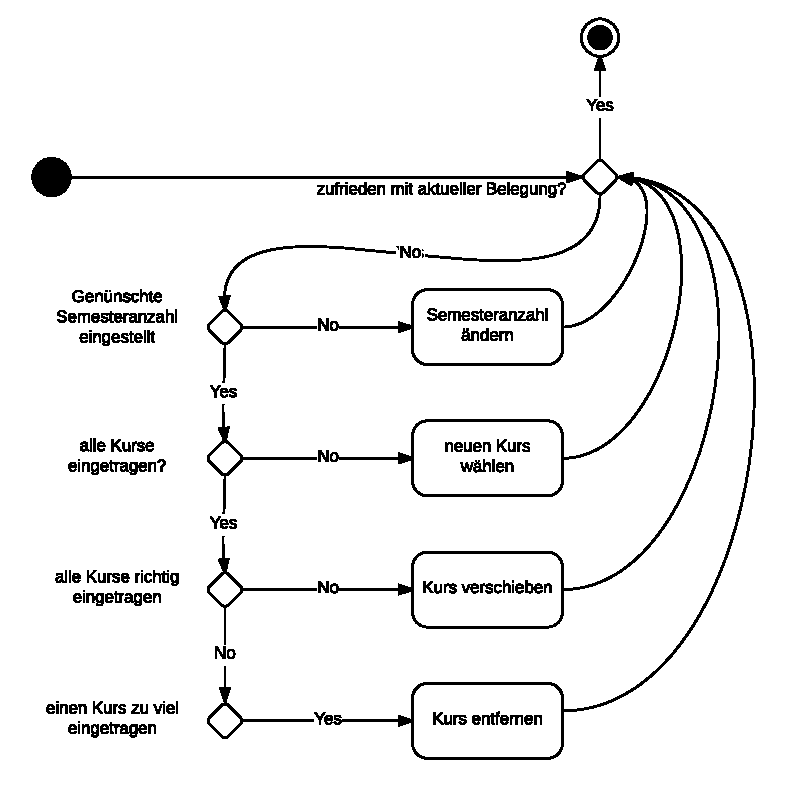
\includegraphics[width=0.8\textwidth]{figures/180_Belegungaendern_aktivitaet.pdf}
\caption{Aktivitätsdiagram vom Use Case Belegung wählen}
\end{figure}

\subsection{Logik Coverage}
Source Code
Wirtschaftsregel -- Cacc

Specifikation: Vertiefungsgebiete 


\subsection{Input}
Input von verschiedenen Helfermethoden, wie Kartesisches Produkt mit richtiger Partitionierung

\end{document}
